% =====================================================================
% Semana 1 · S1.2 — Red serie, KVL y balance de potencia
% Fundamentos de Sistemas Electrónicos Analógicos (Ingeniería Aeroespacial)
% Compilar: pdflatex semana_1_s12_serie_kvl_balance.tex  (2 pasadas)
% =====================================================================
\documentclass[aspectratio=169]{beamer}

\usepackage[utf8]{inputenc}
\usepackage[T1]{fontenc}
\usepackage{lmodern}
\usepackage[spanish,es-tabla]{babel}
\usepackage{amsmath,amssymb}
\usepackage{siunitx}
\usepackage{booktabs}
\usepackage{microtype}
\usepackage{circuitikz}

% ---- Paleta del curso (navy/gold) ------------------------------------
\definecolor{navy}{RGB}{23,54,93}       % 17365D
\definecolor{navysoft}{RGB}{72,101,140}
\definecolor{gold}{RGB}{179,142,62}     % B38E3E
\definecolor{ink}{RGB}{44,51,58}
\definecolor{soft}{RGB}{244,241,234}    % F4F1EA

\usetheme{default}
\setbeamertemplate{navigation symbols}{}
\setbeamertemplate{footline}[frame number]
\setbeamercolor{structure}{fg=navy}
\setbeamercolor{frametitle}{fg=white,bg=navy}
\setbeamercolor{title}{fg=navy}
\setbeamercolor{subtitle}{fg=navysoft}
\setbeamercolor{itemize item}{fg=gold}
\setbeamercolor{itemize subitem}{fg=gold}
\setbeamercolor{block title}{fg=white,bg=navy}
\setbeamercolor{block body}{bg=soft}
\setbeamercolor{example text}{fg=navy}
\setbeamertemplate{itemize item}{\scriptsize\raise1.25pt\hbox{\donotcoloroutermaths$\bullet$}}
\setbeamertemplate{itemize subitem}{\scriptsize\raise1.25pt\hbox{\donotcoloroutermaths$\circ$}}
\setbeamerfont{frametitle}{size=\large,series=\bfseries}

\title[S1.2 · Serie y balance]{Red serie, KVL y balance de potencia}
\subtitle{S1.2 — Simulaciones y laboratorio de la Semana 1}
\institute{Licenciatura en Ingeniería Aeroespacial\\ UNAM · ENES Unidad Juriquilla}
\author{M. en C. José de Jesús Santana Ramírez}
\date{Semestre 2027-1}

\begin{document}

% ---------------------------------------------------------------------
\begin{frame}[plain]
  \titlepage
\end{frame}

% ---------------------------------------------------------------------
\begin{frame}{Objetivos de la sesión}
  \begin{itemize}
    \item Definir una conexión \textbf{en serie} y sus tres propiedades inmediatas.
    \item Aplicar la \textbf{Ley de tensiones de Kirchhoff (KVL)} con signos correctos.
    \item Deducir el \textbf{divisor de tensión}: $V_{Rk} = V_{in}\cdot R_k/R_t$.
    \item Usar la \textbf{convención pasiva de signos} y verificar el \textbf{balance de potencia} $\sum P = 0$.
    \item Desarrollar por completo el ejercicio de la red $1\,\text{k}\Omega$ + $2.2\,\text{k}\Omega$ + $3.3\,\text{k}\Omega$ a \SI{12}{\volt}.
  \end{itemize}
  \pause
  \begin{block}{Método de trabajo (las 4 acciones de toda simulación)}
    \textbf{Predecir} el signo y el orden de magnitud $\rightarrow$ \textbf{calcular} a mano $\rightarrow$ \textbf{simular} en LTspice $\rightarrow$ \textbf{explicar} diferencias.
  \end{block}
\end{frame}

% ---------------------------------------------------------------------
\begin{frame}{Teoría 1 · ¿Qué es una conexión en serie?}
  Dos o más elementos están \textbf{en serie} cuando por ellos circula la
  \textbf{misma corriente}: la salida de uno se conecta a la entrada del
  siguiente, sin ramas intermedias.

  \begin{columns}[T]
    \begin{column}{0.55\textwidth}
      \resizebox{\linewidth}{!}{%
      \begin{circuitikz}[american voltages, scale=1.1]
        \draw (0,3) to[V, l=$V_{in}$, i=$I$] (0,0);
        \draw (0,3) -- (1.4,3) to[R, l=$R_1$] (3.6,3);
        \draw (3.6,3) -- (4.0,3) to[R, l=$R_2$] (6.2,3);
        \draw (6.2,3) -- (6.6,3) to[R, l=$R_3$] (8.8,3);
        \draw (8.8,3) -- (9.6,3) -- (9.6,0) -- (0,0);
      \node[ground] at (0,0) {};
      \end{circuitikz}}
    \end{column}
    \begin{column}{0.43\textwidth}
      \begin{itemize}
        \item Corriente única: $I = I_{R1} = I_{R2} = I_{R3}$.
        \item Resistencia total: $R_t = R_1 + R_2 + R_3$.
        \item La tensión de la fuente se \textbf{reparte} entre los elementos.
      \end{itemize}
    \end{column}
  \end{columns}
\end{frame}

% ---------------------------------------------------------------------
\begin{frame}{Teoría 2 · Ley de tensiones de Kirchhoff (KVL)}
  \begin{block}{Enunciado}
    La suma algebraica de las tensiones a lo largo de cualquier \textbf{malla
    cerrada} es cero: $\displaystyle\sum V_{malla} = 0$.
  \end{block}
  \pause
  Aplicada a la red serie:
  \[
    V_{in} - V_{R1} - V_{R2} - V_{R3} = 0
    \qquad\Longleftrightarrow\qquad
    V_{in} = V_{R1} + V_{R2} + V_{R3}
  \]
  \pause
  \begin{itemize}
    \item Se recorre la malla en un sentido fijo y se \textbf{resta} toda caída en el sentido de la corriente.
    \item No es una aproximación: la tensión es una \emph{diferencia de potencial}; al cerrar la malla se vuelve al potencial de partida.
  \end{itemize}
\end{frame}

% ---------------------------------------------------------------------
\begin{frame}{Teoría 3 · Divisor de tensión}
  Con $I = V_{in}/R_t$, la caída en la resistencia $k$ es:
  \[
    V_{Rk} = I\cdot R_k = V_{in}\cdot\frac{R_k}{R_t}
  \]
  \pause
  \begin{itemize}
    \item La fracción $R_k/R_t$ dice qué parte de la tensión se queda en cada elemento.
    \item \textbf{El elemento de mayor resistencia recibe la mayor caída.}
    \item Aplicación inmediata: predecir el orden de magnitud \emph{antes} de calcular.
  \end{itemize}
\end{frame}

% ---------------------------------------------------------------------
\begin{frame}{Teoría 4 · Convención pasiva de signos}
  \begin{table}
    \begin{tabular}{lll}
      \toprule
      Elemento & Corriente & Potencia $P = V\cdot I$ \\
      \midrule
      \textbf{Pasivo} (resistor) & entra por el terminal $+$ & $P > 0$: \textbf{absorbe} (disipa calor) \\
      \textbf{Activo} (fuente)   & sale por el terminal $+$ & $P < 0$: \textbf{entrega} energía \\
      \bottomrule
    \end{tabular}
  \end{table}
  \pause
  \begin{alertblock}{Clave}
    En LTspice, $I(V_1)$ es la corriente que \textbf{entra} al terminal positivo
    de la fuente: para una fuente que entrega, $I(V_1) < 0$ y $V\cdot I(V_1) < 0$.
    Por eso el balance se escribe $P_{absorbida} + P_{disipada} \approx 0$.
  \end{alertblock}
\end{frame}

% ---------------------------------------------------------------------
\begin{frame}{Teoría 5 · Balance de potencia}
  Conservación de la energía en el circuito:
  \[
    \boxed{\;\sum P = 0 \qquad\Longleftrightarrow\qquad
      P_{fuente}\ (\text{entregada}) = P_{R1} + P_{R2} + P_{R3}\;}
  \]
  \pause
  \begin{itemize}
    \item Es la verificación más directa de que un cálculo (o una simulación) es consistente.
    \item Si la fuente entrega \SI{22.15}{\milli\watt} y los resistores no absorben esa misma cantidad: un valor, un signo o un nodo está mal.
    \item El residual numérico en LTspice es del orden de \num{e-9}: ruido de punto flotante, no error.
  \end{itemize}
\end{frame}

% ---------------------------------------------------------------------
\begin{frame}{Ejercicio · Enunciado}
  \begin{block}{Red serie del laboratorio y de la simulación S1.2}
    \centering
    $V_{in} = \SI{12}{\volt}$, \quad $R_1 = \SI{1}{\kilo\ohm}$,
    $R_2 = \SI{2.2}{\kilo\ohm}$, \quad $R_3 = \SI{3.3}{\kilo\ohm}$.
  \end{block}
  \begin{center}
    \begin{circuitikz}[american voltages, scale=0.95]
      \draw (0,3) to[V, l={$V_{in}=12\,\mathrm{V}$}, i=$I$] (0,0);
      \draw (0,3) -- (2,3) to[R, l={$R_1=1\,\mathrm{k}\Omega$}] (4,3);
      \draw (4,3) -- (4.4,3) to[R, l={$R_2=2.2\,\mathrm{k}\Omega$}] (6.8,3);
      \draw (6.8,3) -- (7.2,3) to[R, l={$R_3=3.3\,\mathrm{k}\Omega$}] (9.6,3);
      \draw (9.6,3) -- (10.4,3) -- (10.4,0) -- (0,0);
    \node[ground] at (0,0) {};
    \end{circuitikz}
  \end{center}
  \textbf{Determinar:} $R_t$, $I$, $V_{R1}$, $V_{R2}$, $V_{R3}$, $P_1$, $P_2$, $P_3$,
  y decidir si los resistores de \SI{0.25}{\watt} cumplen derating de 50\,\%.
\end{frame}

% ---------------------------------------------------------------------
\begin{frame}{Desarrollo del ejercicio · Paso 1 — Resistencia total}
  \[
    R_t = R_1 + R_2 + R_3 = 1\,\text{k}\Omega + 2.2\,\text{k}\Omega + 3.3\,\text{k}\Omega
  \]
  \[
    \boxed{\;R_t = \SI{6.5}{\kilo\ohm}\;}
  \]
  \pause
  \begin{itemize}
    \item \textbf{Predicción:} $R_t$ debe ser mayor que la mayor resistencia ($3.3\,\text{k}\Omega$). Se cumple: $6.5 > 3.3$ \checkmark
    \item Unidades: al sumar kiloohmios el resultado queda en kiloohmios.
  \end{itemize}
\end{frame}

% ---------------------------------------------------------------------
\begin{frame}{Desarrollo del ejercicio · Paso 2 — Corriente}
  Por Ohm sobre la red completa:
  \[
    I = \frac{V_{in}}{R_t} = \frac{\SI{12}{\volt}}{\SI{6.5}{\kilo\ohm}}
    = \frac{12}{6500}\ \text{A}
  \]
  \[
    \boxed{\;I = \SI{1.846}{\milli\ampere}\;}
  \]
  \pause
  \begin{itemize}
    \item \textbf{Predicción:} del orden de miliamperios (12 V sobre miles de ohmios). \checkmark
    \item Esta es \textbf{la misma corriente} en R1, R2 y R3 (serie).
  \end{itemize}
\end{frame}

% ---------------------------------------------------------------------
\begin{frame}{Desarrollo del ejercicio · Paso 3 — Caídas de tensión}
  \begin{align*}
    V_{R1} &= I\cdot R_1 = \SI{1.846}{\milli\ampere}\cdot \SI{1}{\kilo\ohm}
              = \SI{1.846}{\volt}\\[2pt]
    V_{R2} &= I\cdot R_2 = \SI{1.846}{\milli\ampere}\cdot \SI{2.2}{\kilo\ohm}
              = \SI{4.062}{\volt}\\[2pt]
    V_{R3} &= I\cdot R_3 = \SI{1.846}{\milli\ampere}\cdot \SI{3.3}{\kilo\ohm}
              = \SI{6.092}{\volt}
  \end{align*}
  \pause
  \begin{itemize}
    \item O bien con el divisor: $V_{R3} = 12\cdot \frac{3.3}{6.5} = \SI{6.092}{\volt}$ (50.8\,\% de $V_{in}$).
    \item \textbf{Predicción cumplida:} la mayor resistencia tiene la mayor caída.
  \end{itemize}
\end{frame}

% ---------------------------------------------------------------------
\begin{frame}{Desarrollo del ejercicio · Paso 4 — Verificación KVL}
  \[
    V_{R1} + V_{R2} + V_{R3}
    = \SI{1.846}{\volt} + \SI{4.062}{\volt} + \SI{6.092}{\volt}
    = \SI{12.000}{\volt} = V_{in}
    \qquad\checkmark
  \]
  \pause
  \begin{block}{Interpretación}
    La KVL \textbf{cierra exactamente} porque las tres caídas se calcularon con la
    misma corriente. En la práctica real, la suma aproxima 12 V y la diferencia
    es el error de medición del multímetro.
  \end{block}
\end{frame}

% ---------------------------------------------------------------------
\begin{frame}{Desarrollo del ejercicio · Paso 5 — Potencias}
  \begin{align*}
    P_1 &= I^2\,R_1 = (1.846\,\text{mA})^2\cdot 1\,\text{k}\Omega = \SI{3.41}{\milli\watt}\\[2pt]
    P_2 &= I^2\,R_2 = (1.846\,\text{mA})^2\cdot 2.2\,\text{k}\Omega = \SI{7.50}{\milli\watt}\\[2pt]
    P_3 &= I^2\,R_3 = (1.846\,\text{mA})^2\cdot 3.3\,\text{k}\Omega = \SI{11.25}{\milli\watt}
  \end{align*}
  \pause
  \begin{itemize}
    \item \textbf{En serie, $P \propto R$}: el de mayor valor disipa más ($P_3 > P_2 > P_1$).
    \item Cuidado: cada resistor usa \emph{su propia} caída; $P = V_{in}^2/R_k$ sería un error de casi 9$\times$.
  \end{itemize}
\end{frame}

% ---------------------------------------------------------------------
\begin{frame}{Desarrollo del ejercicio · Paso 6 — Balance de potencia}
  \begin{align*}
    \sum P &= P_1 + P_2 + P_3
             = \SI{3.41}{\milli\watt} + \SI{7.50}{\milli\watt} + \SI{11.25}{\milli\watt}
             = \SI{22.15}{\milli\watt}\\[4pt]
    P_{fuente} &= V_{in}\cdot I = \SI{12}{\volt}\cdot \SI{1.846}{\milli\ampere}
                 = \SI{22.15}{\milli\watt}
  \end{align*}
  \[
    \boxed{\;P_{fuente} = \sum P \qquad\checkmark\;}
  \]
  \pause
  \begin{itemize}
    \item La fuente entrega exactamente lo que disipan las tres resistencias.
    \item En LTspice: $V(vin)\cdot I(V1)$ será \textbf{negativo} (\SI{-22.15}{\milli\watt}); el balance se cierra sumando con signo.
  \end{itemize}
\end{frame}

% ---------------------------------------------------------------------
\begin{frame}{Desarrollo del ejercicio · Paso 7 — Derating}
  \begin{itemize}
    \item Resistor de $\SI{0.25}{\watt}$ con derating de 50\,\%: límite de diseño
      \[
        P_{derated} = 0.5\cdot P_{nominal} = \SI{0.125}{\watt} = \SI{125}{\milli\watt}
      \]
    \item Peor caso de la red: $P_3 = \SI{11.25}{\milli\watt}$.
  \end{itemize}
  \[
    \text{margen} = \frac{125}{11.25} \approx 11\times
  \]
  \begin{block}{Decisión de diseño}
    $P_3$ usa menos del 10\,\% del límite con derating $\rightarrow$ \textbf{aceptado
    con amplio margen}. (Comparar: en S1.1, el mismo resistor a \SI{12}{\volt} con
    $1\,\text{k}\Omega$ disipa \SI{144}{\milli\watt} y \emph{sí} excede el límite.)
  \end{block}
\end{frame}

% ---------------------------------------------------------------------
\begin{frame}[fragile]{Verificación en LTspice}
  Abrir \texttt{semana1\_02\_kvl\_serie.asc}, ejecutar \texttt{.op} y consultar
  \texttt{View > SPICE Error Log}. El esquema ya mide $I$, las caídas y el error
  de KVL; para cerrar el balance agregar:

  \begin{verbatim}
.meas op P_R1_mW PARAM I(R1)*I(R1)*1k*1e3
.meas op P_R2_mW PARAM I(R2)*I(R2)*2.2k*1e3
.meas op P_R3_mW PARAM I(R3)*I(R3)*3.3k*1e3
.meas op P_fuente_mW PARAM V(vin)*(-I(V1))*1e3
.meas op Balance_mW PARAM P_fuente_mW-(P_R1_mW+P_R2_mW+P_R3_mW)
  \end{verbatim}

  \textbf{Criterio de éxito:} \texttt{KVL\_error\_uV} $\approx 0$ y
  \texttt{Balance\_mW} $\approx 0$.
\end{frame}

% ---------------------------------------------------------------------
\begin{frame}{Resultado de la simulación}
  \begin{center}
    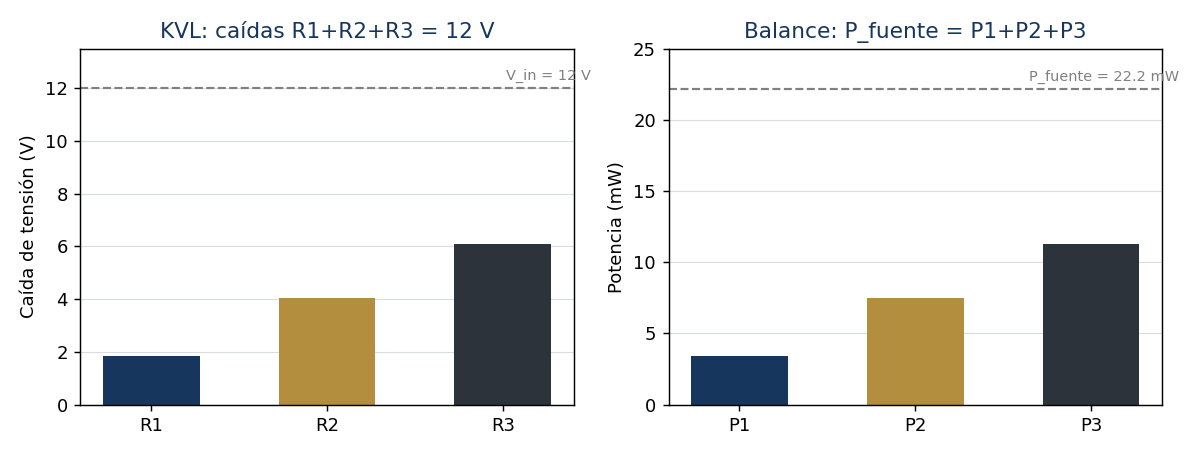
\includegraphics[width=0.82\textwidth]{figs/s12_kvl_balance.png}
  \end{center}
  \begin{itemize}
    \item \textbf{KVL:} $V_{R1}+V_{R2}+V_{R3} = 12.00\,\text{V} = V_{in}$: la malla cierra exactamente.
    \item \textbf{Balance de potencia:} $P_{fuente} = 22.15\,\text{mW} = P_1+P_2+P_3$: la energía se conserva.
    \item \textbf{La mayor caída (y potencia) está en $R_3 = 3.3\,\text{k}\Omega$}: en serie, $P \propto R$.
  \end{itemize}
\end{frame}

% ---------------------------------------------------------------------
\begin{frame}{Errores comunes}
  \begin{table}
    \small
    \begin{tabular}{p{0.32\textwidth}p{0.30\textwidth}p{0.32\textwidth}}
      \toprule
      Error & Consecuencia & Corrección \\
      \midrule
      Sumar caídas con signos arbitrarios & KVL no cierra & Fijar sentido de recorrido y restar toda caída \\
      $P = V_{in}^2/R_k$ en cada resistor & Potencias $\approx 9\times$ mayores & Cada resistor usa \emph{su} caída \\
      Confundir entrega y absorción & Balance con signo invertido & Convención pasiva \\
      Esperar que el menor resistor disipe más & Conclusión de diseño errónea & En serie $P \propto R$ \\
      \bottomrule
    \end{tabular}
  \end{table}
\end{frame}

% ---------------------------------------------------------------------
\begin{frame}{Lectura aeroespacial}
  \begin{itemize}
    \item \textbf{Presupuesto de potencia del EPS:} la auditoría $\sum P = 0$ es la
      misma del satélite: lo que producen los paneles (o entrega la batería) debe
      ser exactamente lo que consumen los subsistemas.
    \item \textbf{Caídas en el arnés:} cable, conector y contacto añaden caídas en
      serie (KVL): un bus de 28 V puede llegar al equipo con 27 V. El arnés se
      dimensiona para que su caída quede dentro del rango aceptado por la carga.
    \item \textbf{Batería carga/descarga:} con convención pasiva, la batería absorbe
      al cargarse ($P>0$) y entrega al alimentar la computadora de vuelo ($P<0$).
      Malos signos $\rightarrow$ batería mal dimensionada.
    \item \textbf{KVL en el WCCA:} repetir la malla con valores extremos
      (tolerancias, deriva) y verificar que siga cerrando antes de validar el diseño.
  \end{itemize}
\end{frame}

% ---------------------------------------------------------------------
\begin{frame}{Preguntas de verificación}
  \begin{enumerate}
    \item Si $V_{in}$ sube de 12 V a 14 V, ¿en qué \% cambia la corriente y la potencia total?
      \uncover<2->{\emph{(Corriente +16.7\,\%; potencia +36\,\% porque $P\propto V^2$.)}}
    \item ¿Qué caída es mayor, la de $R_1$ o la de $R_3$, y por qué?
    \item ¿Por qué $V(vin)\cdot I(V1)$ sale negativo en el log de LTspice?
    \item Un resistor de $\SI{0.25}{\watt}$ disipa 0.2 W continuos: ¿cumple derating de 50\,\%?
      \uncover<3->{\emph{(No: $0.2 > 0.125$ W $\rightarrow$ rechazado; subir a $\SI{0.5}{\watt}$.)}}
    \item ¿Por qué el balance de potencia es una \emph{verificación} y no una ley aparte?
      \uncover<4->{\emph{(Es la conservación de la energía aplicada al circuito.)}}
  \end{enumerate}
\end{frame}


\end{document}
